
\begin{figure}[h]
 \centering
 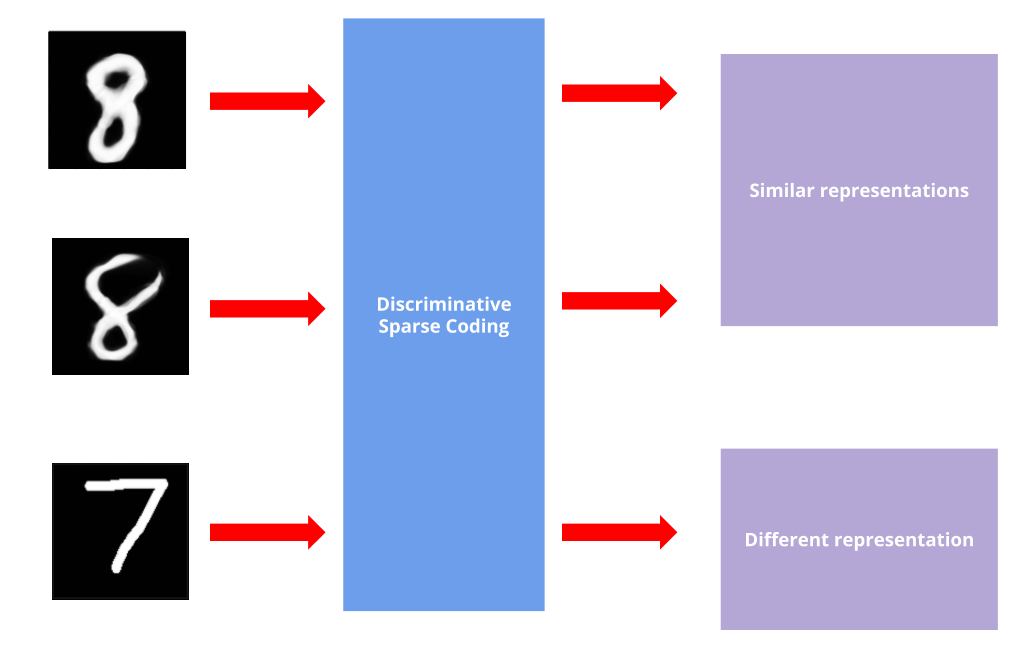
\includegraphics[scale=0.3]{discriminative.png}
 % discriminative.png: 1029x662 px, 72dpi, 36.30x23.35 cm, bb=0 0 1029 662
 \caption{Objective of discriminative Sparse Coding}
 \label{fig:discriminative}
\end{figure}
Generally, to get a discriminative sparse code, the first need is a discriminative dictionary. Indeed,  during the sparse coding step, if the dictionary is discriminative, the minimization of the lost function will tend to create the sparse code using the right atoms and be disadvantaged for the others atoms in term of reconstruction. The result will be a discriminative sparse code.\\
However, most methods of discriminative sparse coding are not unsupervised, because they use the label information during the training of the dictionary. \cite{8294264} enumerate some of these methods:
%One way to have discriminative Sparse coefficients is firstly to have a discriminative dictionary and there are serveral approach for discriminative Dictionary Learning enumerate by \cite{8294264}:
\begin{itemize}
 \item In presence of label:
    \begin{enumerate}
     \item Learn one dictionary per class
     \item Prune large dictionaries
     \item Jointly learn dictionary and classifier
     \item Embed class label into the learning of sparse coefficients
     \item Learn a histogram of dictionary elements over signal constituents
    \end{enumerate}

 \item For weakly supervised:\\
    Several max margin-based, non-convolutive, synthesis dictionary learning approaches
\end{itemize}
For the extraction of our features, we are only interested in two methods. We made this choice because both methods are state-of-the-art of discriminative Sparse Coding for feature's extraction (for classification purposes) and because they are simple to implement. We have chosen:
\begin{itemize}
 \item One Dictionary per class
 \item Embed class label into the learning of sparse coefficients, through a method named \textit{Label constitent K-SVD}.
\end{itemize}


%However in our problem of extract new features for speech we must compare each $\alpha$ with other, thus we must use only one dictionary.
